For trialling the LR Heuristic and observing results for the ESLP we construct 
a test case using UK annual energy demands across different regional authorities
and data on existing UK renewable infrastructure. In this section we outline 
the data collected and processed to setup this test case,
and then describe computational results of the ESLP and LR Heuristic implementations.

\subsection{Data and Processing}\label{sec:data_and_processing}

To obtain proper estimates for the ESLP, we required:

\begin{enumerate}
    \item Demand: Time series of energy demands for different centres across the UK
    \item Setup Costs: Estimates of UK Renewable Energy Site Setup Costs
    \item Supply Site Capacities: Estimates of UK Renewable Energy Site capacities
    \item Supply Costs: Estimates of generation and transmission costs for different UK Renewable Energy 
\end{enumerate}

Item 1 was obtained from public UK government data on annual UK
electricity consumption statistics across 296 regional authorities from 2005 to 2022 \cite{sub_national_electricity_consumption}.
This provided a timeseries of annual electricity demand across different regional authorities.
Items 2 and 3 were obtained from UK government datasets on all current and completed UK Renewable 
Energy Plants construction projects exceeding 1MW (1880 in total). This included site locations,
technology types e.g. Hydro, Wind, Solar, and capacity.
Based on technology types and capacity, an estimate of setup cost was obtained by combining these
with energy setup capital costs for different technology types, obtained from \cite{nalley2022annual}. Annual capacities 
were obtained by scaling capacity up to cover a year.

\begin{equation}
    \text{Setup Cost}_{USD} = \text{Capacity}_{MWh} \times \text{Capital Cost}_{USD KWh^{-1}} \times 1000 
\end{equation}.

Generation costs in item 3 were obtained from \cite{irena2020}, which provides generation costs (USD) per KWH. 
For transmission, we assumed that all transport was done through overhead wires and obtain an estimate
of 0.0258 USD per km per MWh \cite{desantis2021cost}. A cost per unit of energy between any supply and 
demand locations could then be estimated by calculating the geodesic between two locations. \par

We obtained therefore a list of locations and their energy requirements over time, a list of supply sites,
their setup costs and their capacities, and finally an estimate of supply costs between all demand sites and 
supply sites.


\subsection{Implementation}\label{sec:implemenation}
The ESLP and LR Heuristic were both implemented in Pyomo \cite{bynum2021pyomo} 
and solved using the gurobi solver with its default parameters. Initialising the $\lambda$ with $0$ 
resulted in the best results when testing over a grid search, likely because it allowed the LR ESLP 
exploratory freedom that the subgradients could then incrementally adjust.
The option to impose a big M constraint term was also included, although fully investigating the impact of using this wasn't fully investigated in this project.
The complete code can be found at: \href{https://github.com/intimantripp/UK_RenewableEnergy_CFLP}{https://github.com/intimantripp/UK\_RenewableEnergy\_CFLP}


\subsection{Results}
We present the converged solutions, error for the LR Heuristic and performance times for both 
across various different scenarios.
First we present the results on a constructed base case, the purpose of which was to establish that
both the ESLP and LR Heuristic were functioning correctly. We then present 
the results on the UK example described. 

\subsubsection{Base Case}
Two simplified test cases were constructed, both using three demand and three supply sites with
demand varying over 5 years. In the first case the optimal solution was for the closest site to provide
power, in the second this was the case for all but the final year, when it became optimal for one station
to provide all power due to cost increases for the other stations.

Both methods converged on the optimal solutions. These results are conveyed 
below in table \ref{tab:baseline_performance}. Figure \ref{fig:base_cases} shows 
the base case solutions found, which correspond to the designed optimal setups.
The demand fluctuation are not displayed, but the thickness of the lines indicates
the proportion of total energy supplied to each site 
of the total energy over all time periods.
\begin{figure}[H]
    \centering
    \begin{subfigure}[b]{0.45\textwidth}
        \centering
        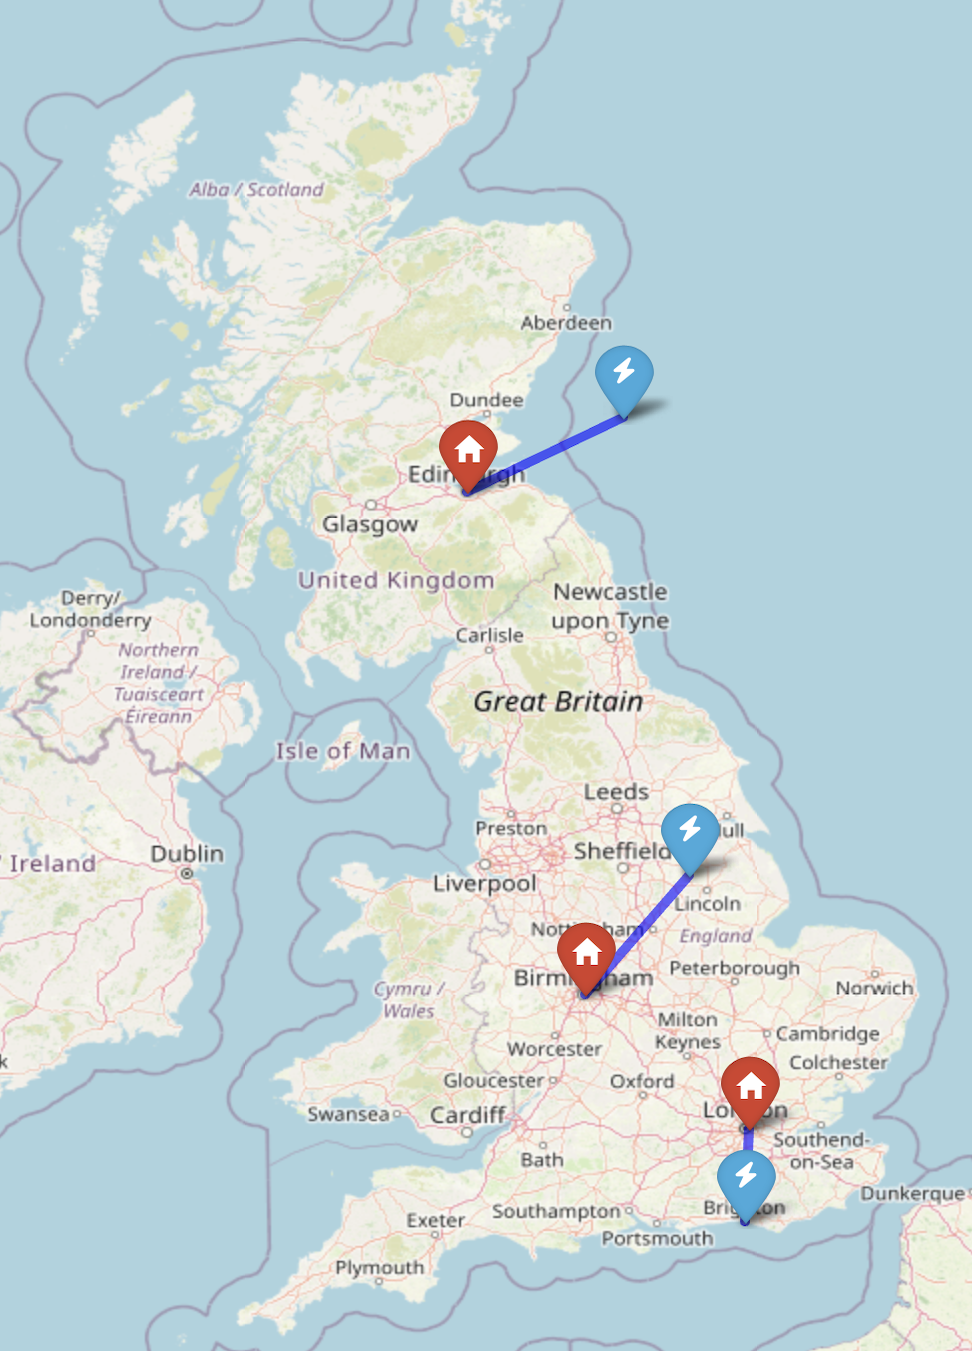
\includegraphics[width=\textwidth]{figures/base_case_1.png}
        \caption{Base Case 1: 3 demand sites each with one optimal supply site over entire time horizon}
        \label{fig:base_case_1}
    \end{subfigure}
    \hfill
    \begin{subfigure}[b]{0.45\textwidth}
        \centering  
        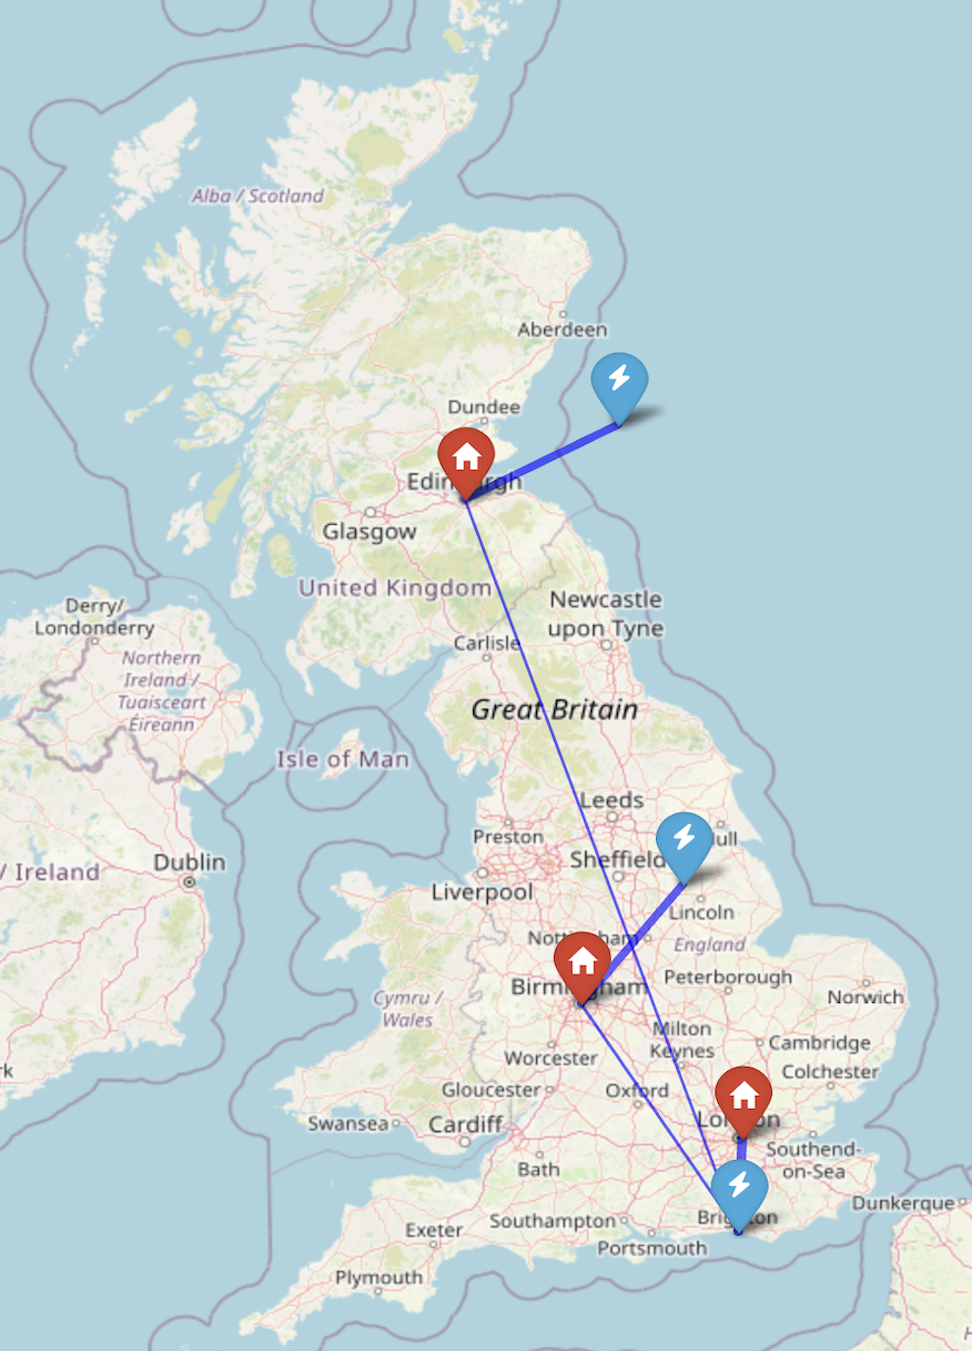
\includegraphics[width=\textwidth]{figures/base_case_2.png}
        \caption{Base Case 2: 3 demand sites each with one optimal supply site over entire time horizon
        except for final timestep}
        \label{fig:base_case_2}
    \end{subfigure}
    \caption{Base Case results compared}
    \label{fig:base_cases}
\end{figure}

\begin{table}[h]
    \centering
    \caption{Performance Comparison of LR Heuristic and to ESLP}
    \label{tab:baseline_performance}
    \renewcommand{\arraystretch}{1.2}
    \setlength{\tabcolsep}{10pt} % Adjust column spacing
    
    \begin{tabular}{l ccc c}
        \toprule
        \textbf{Test Case} & \multicolumn{3}{c}{\textbf{LR Heuristic}} & \textbf{ESLP} \\
        \cmidrule(lr){2-4} \cmidrule(lr){5-5}
         & \textbf{Time (s)} & \textbf{Gap} & \textbf{Iterations} & \textbf{Time (s)} \\
        \midrule
        1 & 0.12 & 0.0 & 1 & 0.14 \\
        2 & 0.14 & 0.0 & 2 & 0.16 \\
        \bottomrule
    \end{tabular}
\end{table}






\subsubsection{UK Energy System}
We varied the number of demand and supply sites to see how the 
different methods scaled across these. The number of years considered was kept constant at 22, 
the full length of data available. Subsets of data obtained were checked for feasibility before 
attempting to solve. The results of trial runs of 
different sizes are show in table \ref{tab:uk_performance}.


\begin{table}[h]
    \centering
    \caption{Performance Comparison of LR Heuristic and to ESLP}
    \label{tab:uk_performance}
    \renewcommand{\arraystretch}{1.2}
    \setlength{\tabcolsep}{10pt} % Adjust column spacing
    
    \begin{tabular}{cc ccc c}
        \toprule
        \textbf{NS} & \textbf{ND} & \multicolumn{3}{c}{\textbf{LR Heuristic}} & \multicolumn{1}{c}{\textbf{ESLP}} \\
        \cmidrule(lr){3-5} \cmidrule(lr){6-6}
         & & \textbf{Time (s)} & \textbf{Gap} & \textbf{Iterations}& \textbf{Time (s)} \\
        \midrule
        3 & 3 & 0.13 & 0 & 1 & 0.13 \\
        10 & 10 & 0.32 & 0.02 & 5 & 0.16\\
        10 & 20 & 5.81 & 0.01 & 8 & 0.22 \\
        10 & 50 & 0.3 & 0.01 & 8 & 0.24\\
        20 & 10 & 9.98  & 0.01 & 23 & 0.18\\
        30 & 10 & 13.77  & 0.02 & 23 & 0.23\\
        50 & 20 & 67.64 & 0.01 & 42 & 0.54 \\
        50 & 50 & 100.16 & 0.02 & 50 & 1.05 \\
        100 & 100 & 600.07& 0.01 & 50 & 4.57 \\
        200 & 200 & 1800.02 & 0.02 & 80 & 20.2 \\

        \bottomrule
    \end{tabular}

    \vspace{5pt}
    \footnotesize NS = Number of Supply Sites, ND = Number of Demand Sites. 
    Gap = (UB - LB)/UB.
\end{table}




The LR Heurisic clearly takes significantly
longer to reach a solution than simply solving
the ESLP directly with the Gurobi solver, scaling poorly regardless of whether
increasing supply sites or demand sites. The LR heuristic 
however did consistently converge to a tighter
bound, and given higher maximum iterations the 
gap continued to narrow in all cases.

We also present some of the figures illustrating the 
power lines the ESLP solutions converged on \ref{fig:uk_cases}. Figures with more sites were
too connected for differing sites to be discernable. 

Some comments on what this model suggested for UK renewable energy infrastructure.
The model favoured Hydro Power stations over any other. This is likely due to 
transmission being relatively cheap, exacerbated by the use of shortest distances 
to arrive at transmission costs, and power generation being cheapest for hydro power stations
alongside large amounts of capacity, even despite their higher setup cost.

\begin{figure}[H]
    \centering
    \begin{subfigure}[b]{0.45\textwidth}
        \centering
        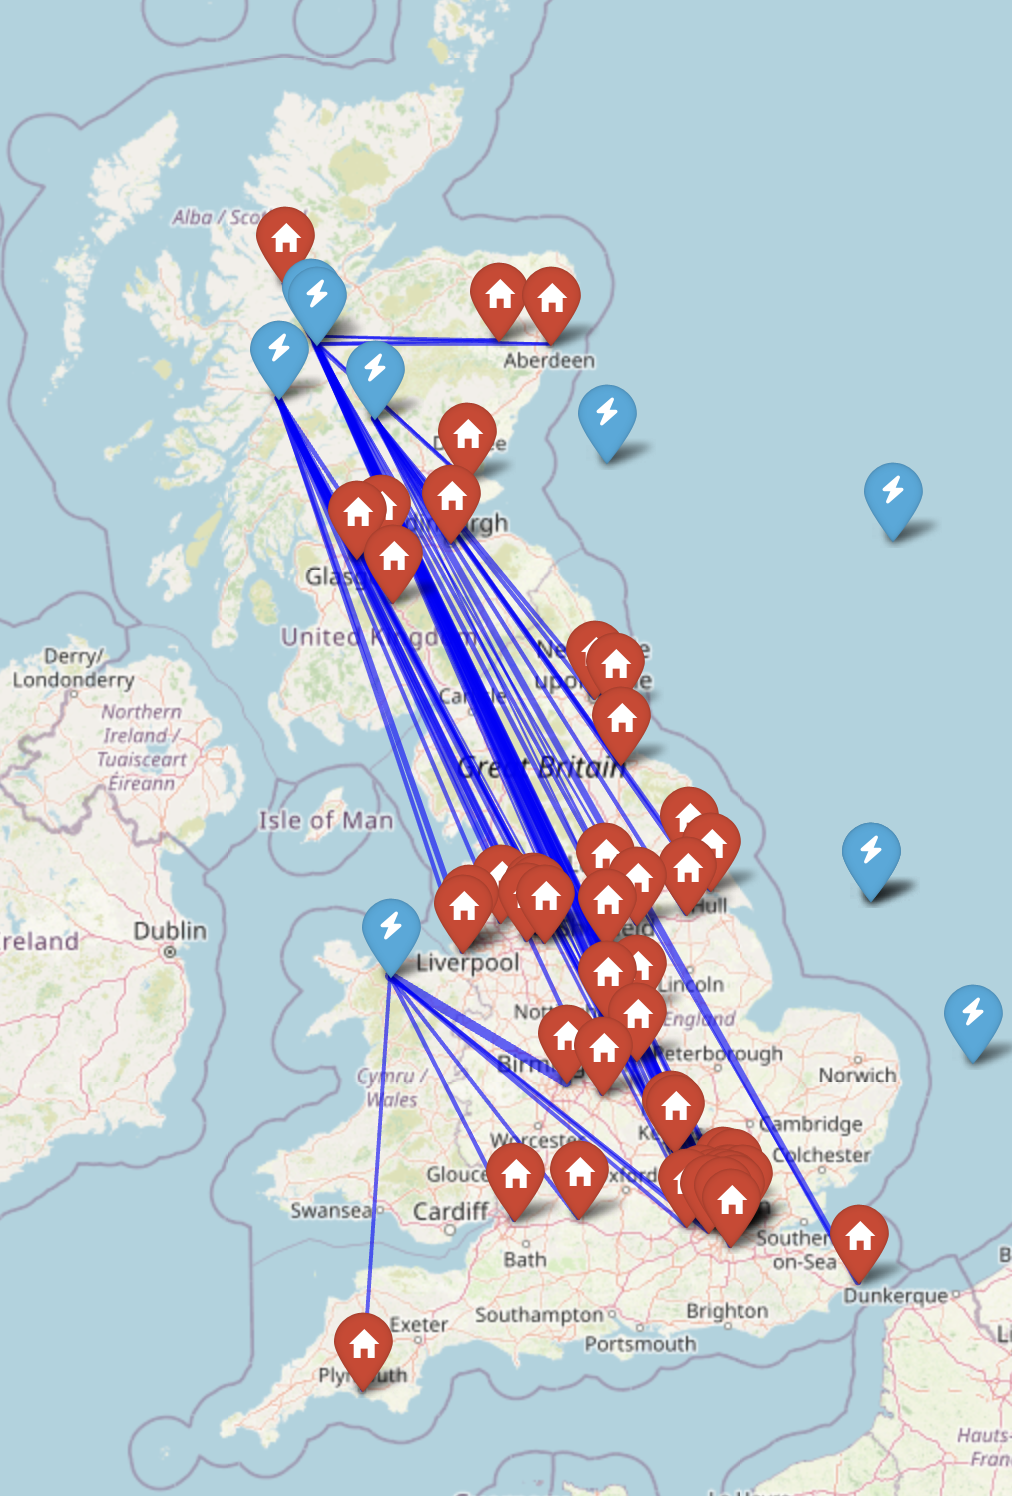
\includegraphics[width=\textwidth]{figures/test_8_base.png}
        \caption{Case with 50 demand sites and 10 supply sites}
        \label{fig:uk_case_1}
    \end{subfigure}
    \hfill
    \begin{subfigure}[b]{0.45\textwidth}
        \centering  
        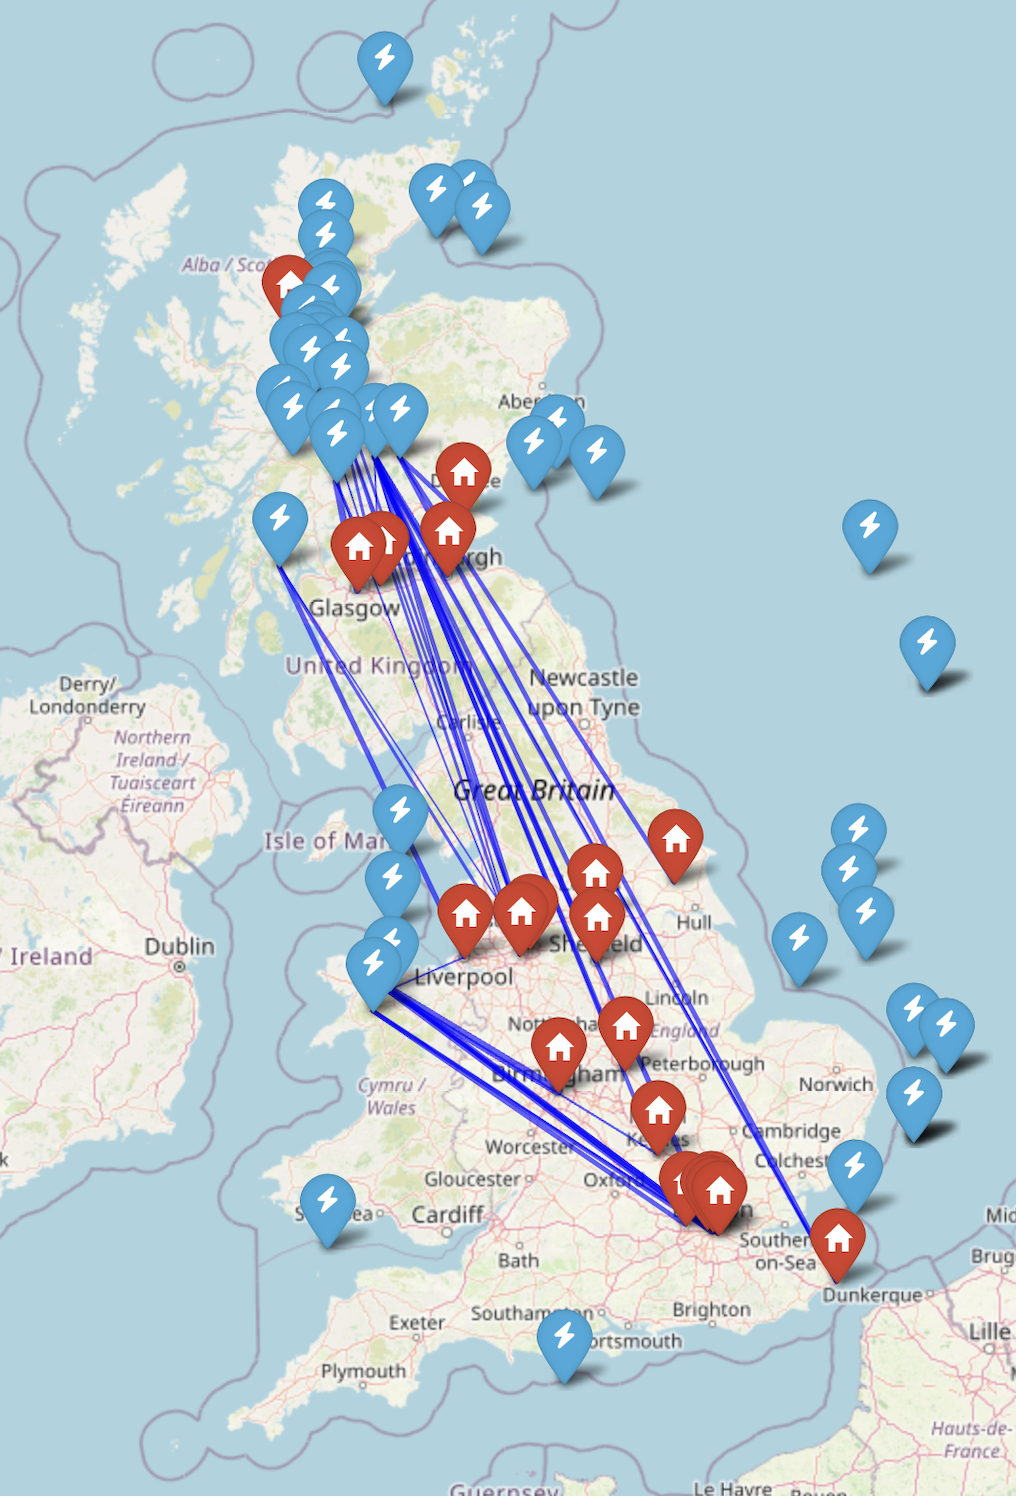
\includegraphics[width=\textwidth]{figures/test_12_base.png}
        \caption{Case with 20 demand sites and 50 supply sites}
        \label{fig:uk_case_2}
    \end{subfigure}
    \caption{UK Energy Networks found as solutions to the ESLP}
    \label{fig:uk_cases}
\end{figure}



\subsection{Future Modifications}\label{sec:future_modifications}
A number of future modifications suggested themselves through this project.

Modifying the subgradient algorithm, for instance by using the r-algorithm as is done in 
\cite{wu2006capacitated} is one possibility, although it is unlikely this would drastically
improve the LR ESLP such that the method becomes comparable to the gurobi solver.

A more interesting modification would be to introduce time-dependency on when sites can be setup, 
rather than assuming all sites are constructed at initiation. This would make such modelling far more
relevant for capital-cost forecasting, as prolonging a site's 
construction until such a time as it is needed could then alter its setup-costs through
time-value-of-money considerations. This could result in more realistic solutions being optimal.
For instance, if demand were expected to rise at some future date at one site drastically, delaying
constructiong to meet the additional demand until it is realised could result in lower
total cost.

A very practical improvement would be to extend this model to consider storage capabilities at different
sites too, incorporating different storage technologies and associated costs and savings in 
utilising them. This could potentially make some facilities like solar and wind more appealing,
although the additional complexity of considering at every site an optimal storage technology
would significantly increase the size of the problem.





